\subsection{Hardware - V2.2(Final)}
\setAuthor{Richard Krammer}


    This section describes the latest hardware of the basic node. The basic node is a 
    simple node that can measure the ambient temperature and control four RGB-LEDs.
    The hardware consists of the following components:

    \begin{itemize}
        \item Microcontroller
        \item Temperature Sensor
        \item LED Indicator
        \item USB-C Connector
        \item 3.3V DC-DC Converter
        \item Module-Connector
    \end{itemize}

    \subsubsection{Microcontroller}
        The basic node uses an ESP32-C3-wroom-02 \cite{noauthor_esp32-c3_2023} microcontroller. 
        It is a low-power, highly integrated Wi-Fi and Bluetooth SoC. In the datasheet 
        it was stated that the MCU is recommended for a wide range of applications, including smart home devices 
        and other IoT products.
        Before the ESP32-C3 was chosen, it was compared with the ESP32-S3-wroom-2 to see which one
        would be the better fit for the basic node. 

        \vspace{0.5cm}
        \begin{Parallel}{0.45\textwidth}{0.45\textwidth}
            \ParallelLText{
            \textbf{ESP32-C3-WROOM-02 :}
            \begin{itemize}
                \item 15 GPIOs
                \item Single-core 32-bit RISC-V CPU up to 160Mhz
                \item 4 or 8 MB flash
                \item PCB antenna  external antenna version
                

            \end{itemize}
            }
            \ParallelRText{ 
            \textbf{ESP32-S3-WROOM-2 :}
            \begin{itemize}
                \item 33 GPIOs
                \item Dual-core 32-bit RISC-V CPU up to 240Mhz
                \item 16 or 32 MB flash
                \item PCB antenna  external antenna version
                
            \end{itemize}
            }
            \ParallelPar
        \end{Parallel}

        \begin{figure}[H]%
            \centering
            \subfloat[\centering ESP-C3]{{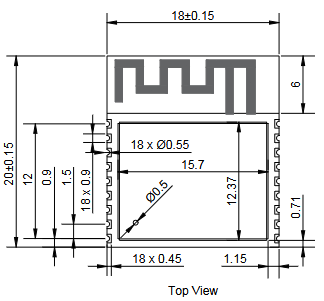
\includegraphics[width=5.5cm]{assets/HW/ESP32-C3-sheet.png} }}%
            \qquad
            \subfloat[\centering ESP-S3]{{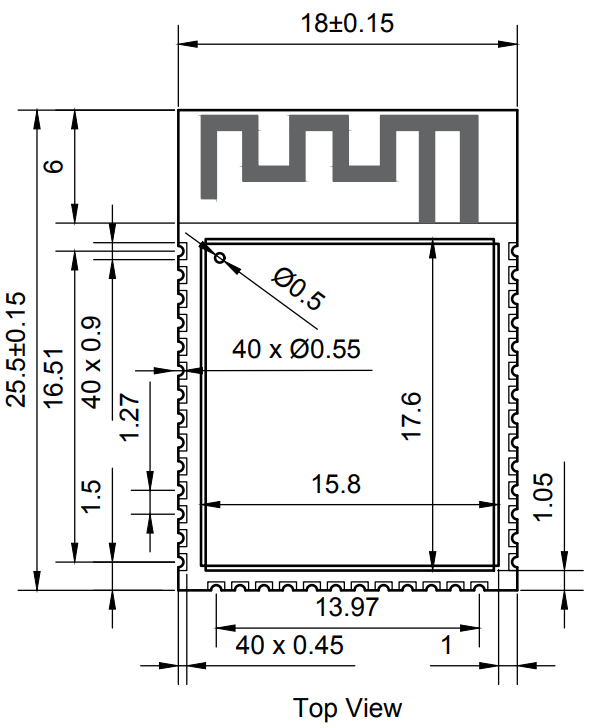
\includegraphics[width=5cm]{assets/HW/ESP-S3-sheet.png} }}%
            \caption{Pyhsical comparison of the ESP32-C3 and ESP32-S3, Unit in mm.}%
            \label{fig:example}%
        \end{figure}

        The ESP32-C3 does not have as many GPIO pins compared to the ESP32-S3, however the 
        abundance of GPIO pins is not necessary for the basic node. The ESP32 C3 is also 
        cheaper and alocates less space on the PCB.

        \begin{figure}[H]
            \centering
            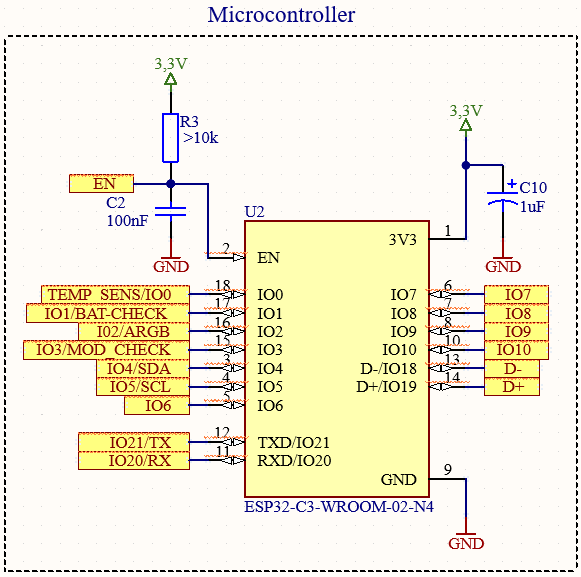
\includegraphics[height = 7.5cm]{assets/HW/ESP32-C3-schematic.png}
            \caption{ESP32-C3 implemented in the schematic.}
        \end{figure}




    \subsubsection{Temperature sensor}
        The DS18B20 was chosen as the temperature sensor. It is a digital thermometer
        with an operating temperature range of -55°C to +125°C. The sensor is connected
        to the microcontroller via GPIO0 and communicates over a 1-Wire bus.
        This sensor was used instead of the DHT11, for being smaller in size.

        \begin{figure}[H]
            \centering
            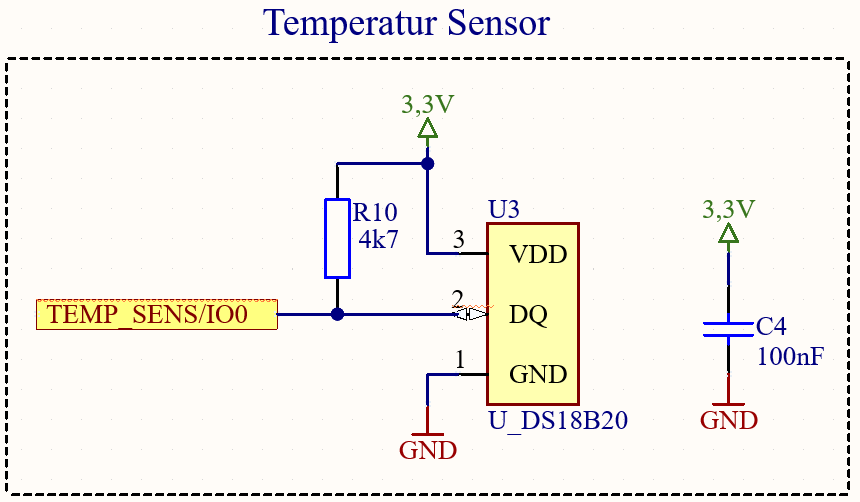
\includegraphics[width=0.7\textwidth]{assets/HW/DS18B20-schematic.png}
            \caption{DS18B20 implemented in the schematic.}
        \end{figure}

    \subsubsection{LED Indicator}
        The basic node has four WS2812b ARGB-LEDs. The LEDs are connected to the 
        microcontroller via GPIO 2. The LEDs are used to indicate the status of the node. 
        For example, the LEDs can be used to indicate the temperature range the node is in
        or to display the charge-level of the battery, when attached.

        \begin{figure}[H]
            \centering
            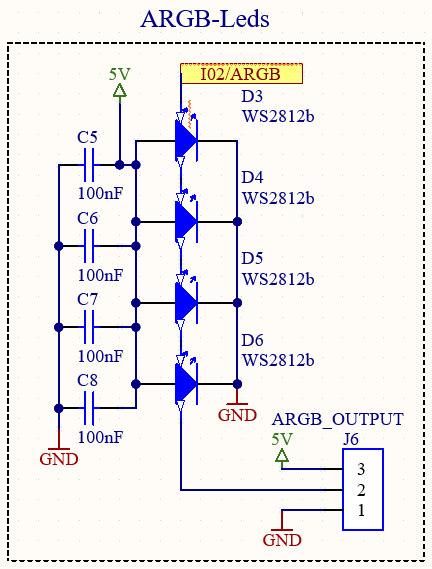
\includegraphics[width=0.4\textwidth]{assets/HW/RGB-LED-schematic.png}
            \caption{RGB-LEDs implemented in the schematic.}
        \end{figure}

    \subsubsection{USB-C Connector}

    The USB-C connector is used to power and programm the basic node. The connector can
    be plugged in both ways, which makes it more user-friendly.

    \begin{figure}[H]
        \centering
        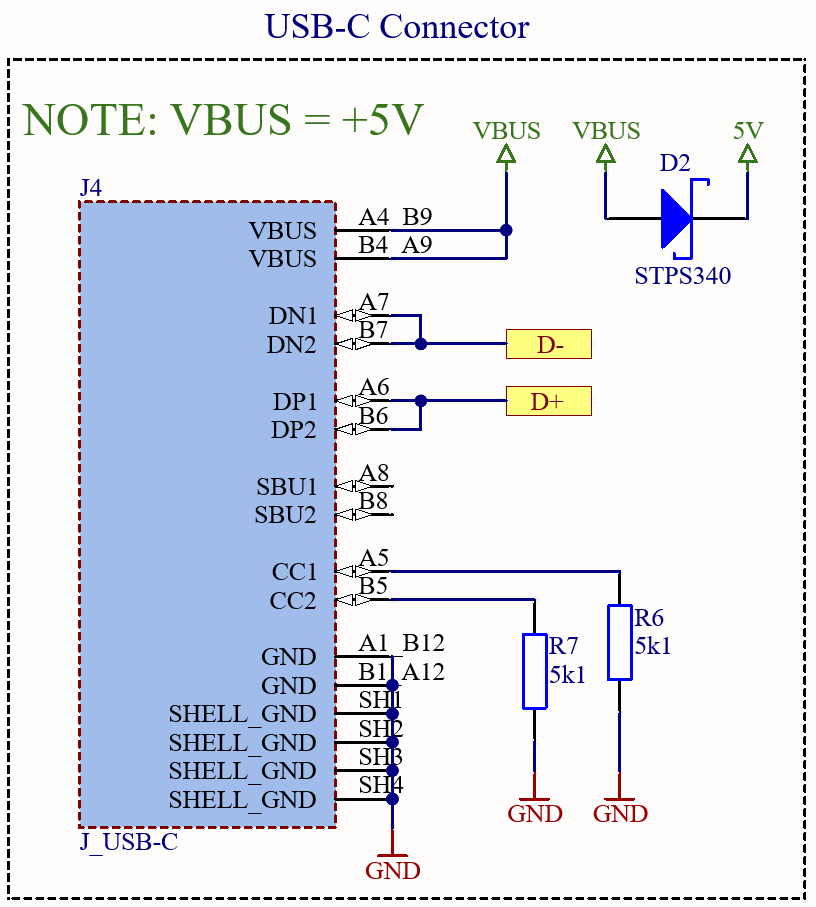
\includegraphics[width=0.4\textwidth]{assets/HW/USB-C-schematic.png}
        \caption{USB-C Connector implemented in the schematic.}
    \end{figure}

    This particular connector was chosen, duo to being the new standard for USB connectors, 
    therefor being widely spread.
    
    The USB protocol interacts with the charger to determine the power output. In order to
    power the basic node with 5V, a 5.1kOhm resistor is connected to the CC1 and CC2 pins.
    The resistor tells the charger that the basic node is a default USB device and can draw
    up to 3A of current.\cite{noauthor_fugen_2023}

    A schottky diode is used to avoid backflow of current.

    \subsubsection{Serial-Port}

    This interface is used to programm the basic node. The interface is connected directly
    with the UART of the ESP32-C3. 

    \begin{figure}[H]
        \centering
        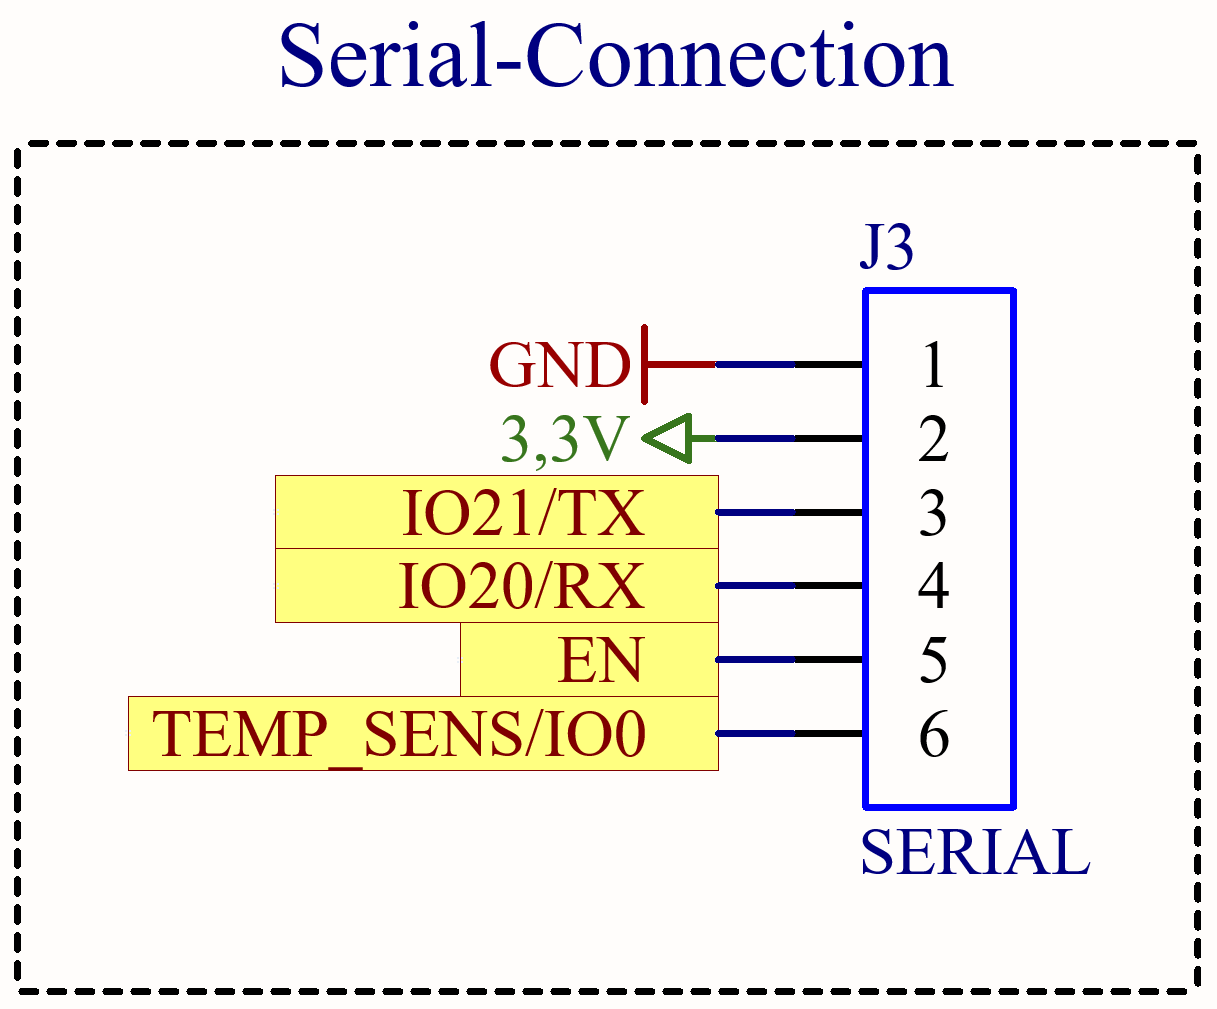
\includegraphics[width=0.4\textwidth]{assets/HW/Serial-Port-schematic.png}
        \caption{Serial-Port implemented in the schematic.}
    \end{figure}
    
    \subsubsection{3.3V DC-DC Converter}

    The  step-down converter TLV62569 from Texas Instruments is used to convert 
    the 5V from the USB-C connector to 3.3V. The converter has a high efficiency
    of up to 95\%, which is significant for battery operation. It powers the
    microcontroller, temperature sensor and a module, if attached to the
    Module-Connector.

    To set the output-voltage, a voltage divider is used. With following formula
    the output voltage can be calculated:

    \begin{equation}
        V_{OUT} = V_{FB} \cdot (1 + \frac{R_1}{R_2})
    \end{equation}

    \begin{figure}[H]
        \centering
        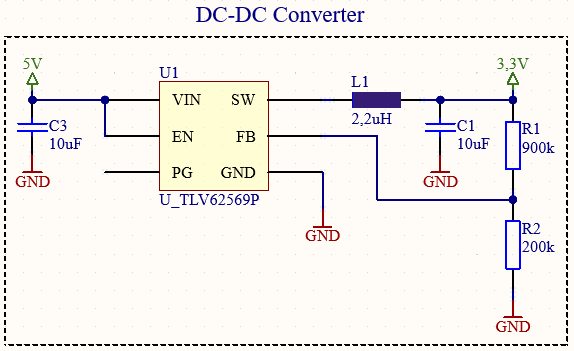
\includegraphics[width=0.7\textwidth]{assets/HW/DC-DC-schematic.png}
        \caption{TLV62569 Converter implemented in the schematic.}
    \end{figure}

    \subsubsection{Module-Connector}

    The module connector is used to join additional modules to the basic module.
    The connector has 15 pins, 8 for power and powermanagment and 7 for 
    communication. 

    \begin{figure}[H]
        \centering
        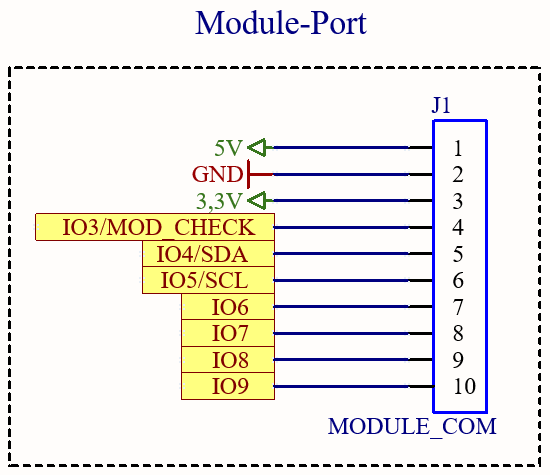
\includegraphics[width=0.4\textwidth]{assets/HW/Module-Connector-schematic.png}
        \caption{Module-Connector implemented in the schematic.}
    \end{figure}

    Pin 3-5 and 6-8 are symmetrical to each other. It was designed this way
    to allow the battery module and motion module to be attached simultaneously.
    The battery module is plugged into pin 1-5 and is connected to following 
    voltages:
    
    \begin{itemize}
        \item 1. VBAT - used to monitor the battery voltage
        \item 2. VBUS - used to charge and disable the battery module when the USB-C 
        is connected
        \item 3. 3V3 - not used, but may be relavant for future modules/revisions
        \item 4. GND
        \item 5. 5V - The battery module powers the basic node over this pin
    \end{itemize}

    Pin 6-15 are used for communication between the modules. 


    \subsubsection{Module-Detection}
    
    The basic node regonizes the attached module by measuring the voltage on pin 9.
    A 100kOhm resistor is installed on the base module pulling pin 9 to GND. 
    When a module is attached, a voltage devider is created. The voltage on pin 9 is 
    determinted by the second resistor on the module. The microcontroller reads the
    voltage and can determine the attached module. 
    
    \begin{figure}[H]
        \centering
        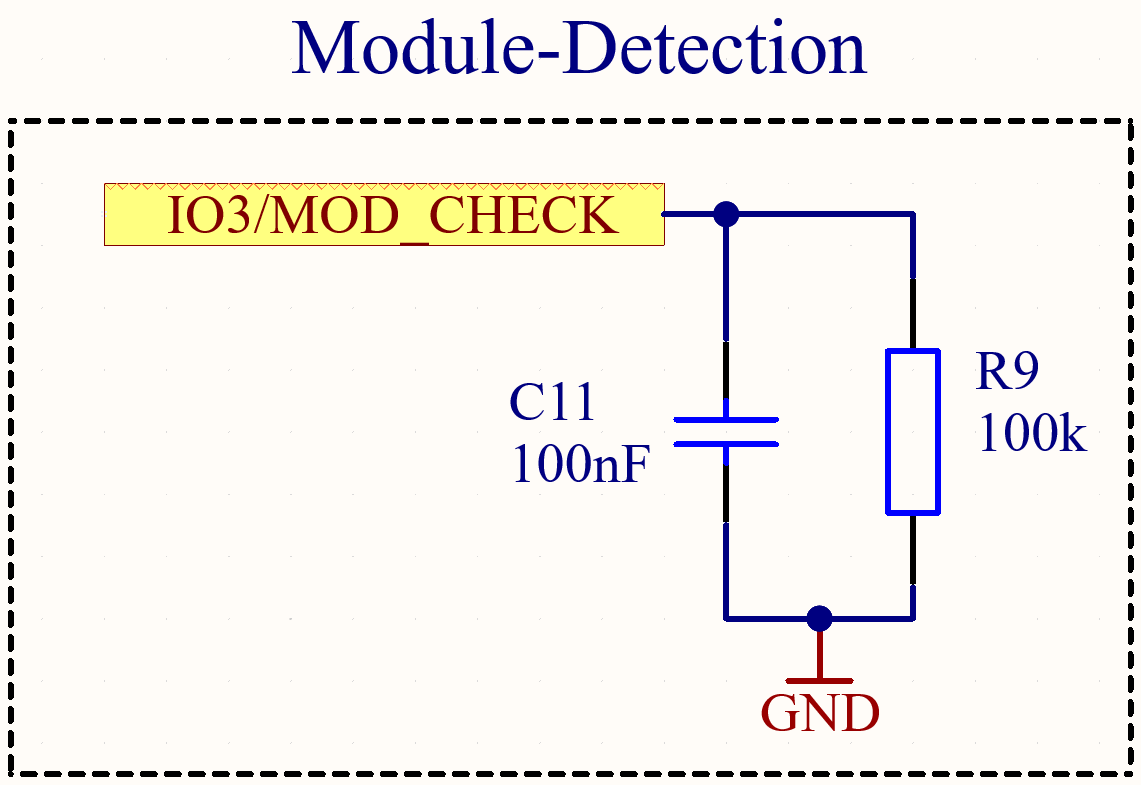
\includegraphics[width=0.4\textwidth]{assets/HW/Module-Detection-schematic.png}
        \caption{Module-Detection implemented on the base module.}
    \end{figure}

    \subsubsection{PCB}

    The PCB has a size of 30x75mm. The compenents used were mainly SMD components, 
    to keep the PCB small. 

    \begin{figure}[H]
        \centering
        
\includegraphics[width=0.7\textwidth]{assets/HW/TBD.png}
        \caption{PCB of the basic node. [Blue - Backside, Red - Frontside]}
    \end{figure}	


